\section{Results}

The results are split in two parts.
The first part is the context switching time value measured by our benchmarking framework.
For the second part, we have measured again the real context switching time with the oscilloscope the same way as for the reference measurement.

\subsection{Internal benchmarking framework results}
The value measured by our internal framework is represented in the table \ref{tab:internal-framework-measurement}.

\begin{table}[!ht]
  \centering
  \begin{tabular}{llll}
  & \multicolumn{3}{c}{Time ($\mu$s)}          \\ \cline{2-4} 
  & \multicolumn{1}{c}{Mean} & Min  & Max  \\ \cline{2-4} 
From task 1 to task 2 & 7812                     & 7812 & 7812 \\
From task 2 to task 1 & 7812                     & 7812 & 7812
\end{tabular}
  \caption{Context switching time measured by our internal benchmarking framework}
  \label{tab:internal-framework-measurement}
  \end{table}

\subsection{External benchmarking framework results}
The context switching time computed by our external framework is displayed in the table \ref{tab:external-framework-measurement}.

\begin{table}[!ht]
  \centering
  \begin{tabular}{llll}
  & \multicolumn{3}{c}{Time ($\mu$s)}                             \\ \cline{2-4} 
  & \multicolumn{1}{c}{Mean} & Min  & \multicolumn{1}{c}{Max} \\ \cline{2-4} 
Context switching time & 18.93                     & 15.62 & 40.26                    \\
\end{tabular}
  \caption{Context switching time measured by our external benchmarking framework}
  \label{tab:external-framework-measurement}
\end{table}

\subsection{Oscilloscope results}
Using the same setup as for the reference measurement, we have measured again the real context switching time with both our internal and external benchmarking framework.

The figure \ref{fig:internal-framework-value-wave} shows the voltage measurement of the two GPIOs used by the tasks while using our internal framework.
The figure \ref{fig:external-framework-value-wave} shows the voltage measurement of the single GPIO used by the external framework while using it.

\begin{figure}[!ht]
  \centering

  \begin{minipage}{0.45\textwidth}
    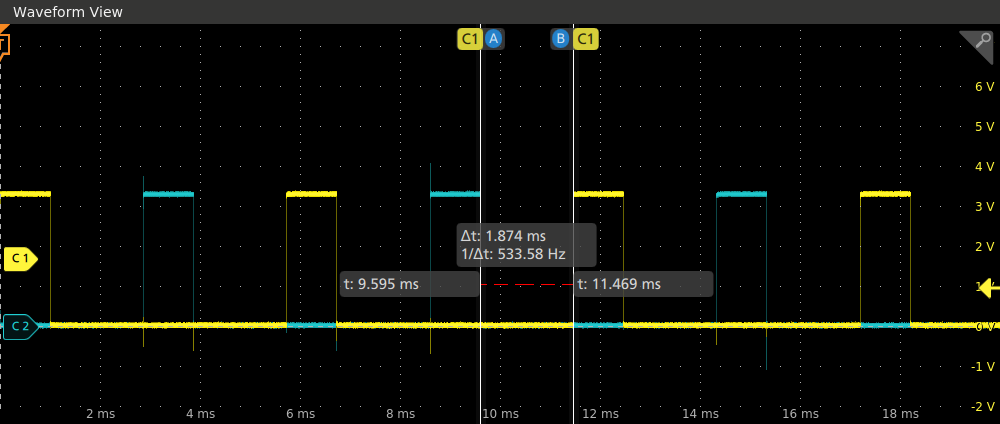
\includegraphics[width=0.9\textwidth]{assets/framework-value-wave.png}
    \caption{\label{fig:internal-framework-value-wave}Internal benchmarking framework voltage measurement}

  \end{minipage}\hfill
  \begin{minipage}{0.45\textwidth}

    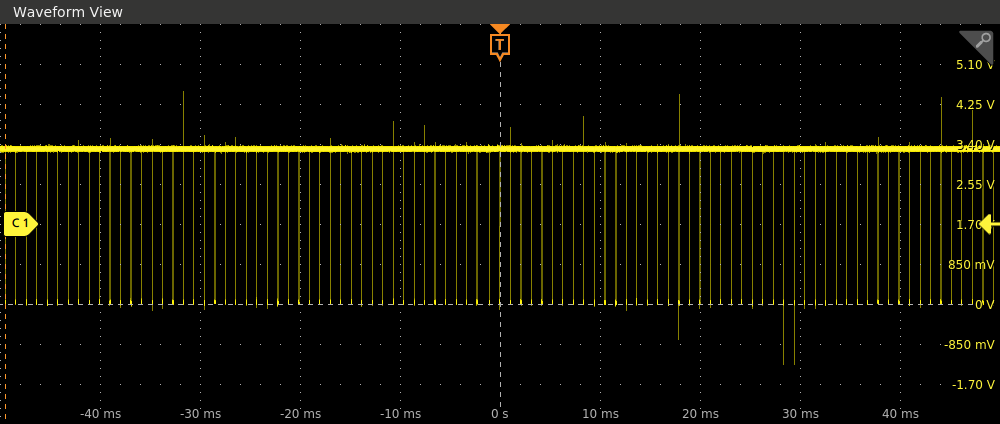
\includegraphics[width=0.9\textwidth]{assets/external-framework-value-wave.png}
    \caption{\label{fig:external-framework-value-wave}External benchmarking framework voltage measurement}

  \end{minipage}
\end{figure}

The table \ref{tab:frameworks-oscilloscope-comparison} shows a comparison of the real context switching time measured with the oscilloscope between the internal framework and the external one.

\begin{table}[!ht]
  \centering
  \begin{tabular}{llllllll}
  & \multicolumn{7}{c}{Time ($\mu$s)}                                                      \\ \cline{2-8} 
  & \multicolumn{3}{c}{Internal framework} &  & \multicolumn{3}{c}{External framework} \\ \cline{2-4} \cline{6-8} 
  & \multicolumn{1}{c}{Mean} & Min  & Max  &  & Mean        & Min         & Max        \\ \cline{2-4} \cline{6-8} 
Context switching time & 1865                     & 1862 & 1866 &  & 14.87       & 14.79       & 14.97      \\
Duration of task 1     & 1003                     & 1003 & 1003 &  & 1003        & 1003        & 1003       \\
Duration of task 2     & 1003                     & 1003 & 1003 &  & 1003        & 1003        & 1003      
\end{tabular}
  \caption{Context switching times and task durations measured with the oscilloscope using our internal and external benchmarking frameworks}
  \label{tab:frameworks-oscilloscope-comparison}
\end{table}
